\subsection{\ShiftsSectionName}

\IFRU{Битовые сдвиги в \CCpp реализованы при помощи операторов $\ll$ и $\gg$.}
{Bit shifts in \CCpp are implemented via $\ll$ and $\gg$ operators.}

\IFRU{Вот этот несложный пример иллюстрирует функцию, считающую количество бит-единиц во входной переменной:}
{Here is a simple example of function, calculating number of $1$ bits in input variable:}

\lstinputlisting{14_bitfields/shifts.c}

\IFRU{В этом цикле, счетчик итераций \IT{i} считает от $0$ до $31$, а $1 \ll i$ будет от $1$ до \TT{0x80000000}. 
Описывая это словами, можно сказать 
\IT{сдвинуть единицу на $n$ бит влево}.
Т.е., в некотором смысле, выражение $1 \ll i$ последовательно выдаст все возможные позиции бит в 32-битном числе. 
Кстати, освободившийся бит справа всегда обнуляется. Макрос \TT{IS\_SET} проверяет наличие этого бита в \TT{a}.}
{In this loop, iteration count value \IT{i} counting from $0$ to $31$, $1 \ll i$ statement will be counting 
from $1$ to \TT{0x80000000}.
Describing this operation in natural language, we would say \IT{shift $1$ by n bits left}.
In other words, $1 \ll i$ statement will consequently produce all possible bit positions in 32-bit number.
By the way, freed bit at right is always cleared. \TT{IS\_SET} macro is checking bit presence in \TT{a}.}

\index{x86!\Instructions!SHL}
\begin{figure}[ht!]
\centering
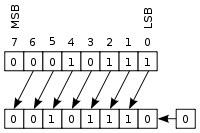
\includegraphics[scale=0.66]{14_bitfields/200px-Rotate_left_logically.png}
\caption{\IFRU{Как работает инструкция \SHL\protect\footnotemark}
{How \SHL instruction works\protect\footnotemark}}
\end{figure}

\footnotetext{\IFRU{иллюстрация взята из}{illustration taken from} wikipedia}

\index{x86!\Instructions!AND}
\IFRU{Макрос \TT{IS\_SET} на самом деле это операция логического И (\IT{AND}) 
и она возвращает ноль если бита там нет, 
либо эту же битовую маску, если бит там есть. 
В \CCpp, конструкция \TT{if()} срабатывает, если выражение внутри её не ноль, пусть хоть $123456$, 
поэтому все будет работать.}
{The \TT{IS\_SET} macro is in fact logical and operation (\IT{AND}) 
and it returns zero if specific bit is absent there,
or bit mask, if the bit is present.
\IT{if()} operator triggered in \CCpp if expression in it isn't zero, it might be even $123456$, that's why
it always working correctly.}

\subsubsection{x86}

\IFRU{Компилируем}{Let's compile} (MSVC 2010):

\lstinputlisting[caption=MSVC 2010]{\IFRU{14_bitfields/shifts_MSVC_ru.asm}{14_bitfields/shifts_MSVC_en.asm}}

\IFRU{Вот так работает SHL (\IT{SHift Left})}{That's how SHL (\IT{SHift Left}) working}.

\IFRU{Скомпилируем то же и в}{Let's compile it in} GCC 4.4.1:

\lstinputlisting[caption=GCC 4.4.1]{14_bitfields/shifts_gcc.asm}

\IFRU{Инструкции сдвига также активно применяются при делении или умножении 
на числа-степени двойки ($1$, $2$, $4$, $8$, итд).}
{Shift instructions are often used in division and multiplications by power of two numbers 
($1$, $2$, $4$, $8$, etc).}

\IFRU{Например:}{For example:}

\begin{lstlisting}
unsigned int f(unsigned int a)
{
	return a/4;
};
\end{lstlisting}

\IFRU{Имеем в итоге}{We got} (MSVC 2010):

\begin{lstlisting}[caption=MSVC 2010]
_a$ = 8							; size = 4
_f	PROC
	mov	eax, DWORD PTR _a$[esp-4]
	shr	eax, 2
	ret	0
_f	ENDP
\end{lstlisting}

\label{SHR}
\index{x86!\Instructions!SHR}
\IFRU{Инструкция \SHR (\IT{SHift Right}) в данном примере сдвигает число на 2 бита вправо. 
При этом, освободившиеся два бита слева (т.е., самые 
старшие разряды), выставляются в нули. А самые младшие 2 бита выкидываются. 
Фактически, эти два выкинутых бита ~--- остаток от деления.}
{\SHR (\IT{SHift Right}) instruction in this example is shifting a number by 2 bits right.
Two freed bits at left (e.g., two most significant bits) are set to zero.
Two least significant bits are dropped.
In fact, these two dropped bits ~--- division operation remainder.}

\index{x86!\Instructions!SHL}
\IFRU{Инструкция \SHR работает так же как и \SHL, только в другую сторону.}
{\SHR instruction works just like as \SHL but in other direction.}

\begin{figure}[ht!]
\centering
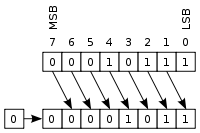
\includegraphics[scale=0.66]{14_bitfields/200px-Rotate_right_logically.png}
\caption{\IFRU{Как работает инструкция \SHR\protect\footnotemark}
{How \SHR instruction works\protect\footnotemark}}
\end{figure}

\footnotetext{\IFRU{иллюстрация взята из}{illustration taken from} wikipedia}

\label{division_by_shifting}
\IFRU{Для того, чтобы это проще понять, представьте себе десятичную систему счисления и число $23$. 
$23$ можно разделить на $10$ просто откинув последний разряд ($3$ ~--- это остаток от деления). 
После этой операции останется $2$ как частное
\footnote{результат деления}.}
{It can be easily understood if to imagine decimal numeral system and number $23$.
$23$ can be easily divided by $10$ just by dropping last digit ($3$ ~--- is division remainder). 
$2$ is leaving after operation as a quotient
\footnote{division result}.}

\IFRU{Так и с умножением. Умножить на $4$ это просто сдвинуть число на 2 бита влево, 
вставив 2 нулевых бита справа (как два самых младших бита). 
Это как умножить $3$ на $100$ ~--- нужно просто дописать два нуля справа.}
{The same story about multiplication.
Multiplication by $4$ is just shifting the number to the left by 2 bits,
while inserting 2 zero bits at right (as the last two bits).
It's just like to multiply $3$ by $100$ ~--- we need just to add two zeroes at the right.}




\subsubsection{ARM + \OptimizingXcode + \ARMMode}

\begin{lstlisting}[caption=\OptimizingXcode + \ARMMode]
                MOV             R1, R0
                MOV             R0, #0
                MOV             R2, #1
                MOV             R3, R0
loc_2E54
                TST             R1, R2,LSL R3 ; set flags according to R1 & (R2<<R3)
                ADD             R3, R3, #1    ; R3++
                ADDNE           R0, R0, #1    ; if ZF flag is cleared by TST, R0++
                CMP             R3, #32
                BNE             loc_2E54
                BX              LR
\end{lstlisting}

\index{ARM!\Instructions!TST}
\TT{TST} \IFRU{это то же что и}{is the same things as} \TEST \IFRU{в}{in} x86.

\index{ARM!Optional operators!LSL}
\index{ARM!Optional operators!LSR}
\index{ARM!Optional operators!ASR}
\index{ARM!Optional operators!ROR}
\index{ARM!Optional operators!RRX}
\index{ARM!\Instructions!MOV}
\index{ARM!\Instructions!TST}
\index{ARM!\Instructions!CMP}
\index{ARM!\Instructions!ADD}
\index{ARM!\Instructions!SUB}
\index{ARM!\Instructions!RSB}
\IFRU{Как я уже указывал}{As I mentioned before}~\ref{shifts_in_ARM_mode}, 
\IFRU{в режиме ARM нет отдельной инструкции для сдвигов.}
{there are no separate shifting instructions in ARM mode.}
\IFRU{Однако, модификаторами}{However, there are modifiers} 
LSL (\IT{Logical Shift Left}), 
LSR (\IT{Logical Shift Right}), 
ASR (\IT{Arithmetic Shift Right}), 
ROR (\IT{Rotate Right}) \IFRU{и}{and} 
RRX (\IT{Rotate Right with Extend}) \IFRU{можно дополнять некоторые инструкции, такие как}
{, which may be added to such instructions as} \MOV, \TT{TST},
\CMP, \ADD, \SUB, \TT{RSB}\footnote{\DataProcessingInstructionsFootNote}.

\IFRU{Эти модифицкаторы указывают, как сдвигать второй операнд, и на сколько.}
{These modificators are defines, how to shift second operand and by how many bits.}

\index{ARM!Optional operators!LSL}
\IFRU{Таким образом, инструкция }{Thus} \TT{``TST R1, R2,LSL R3''} 
\IFRU{здесь работает как}{instruction works here as} $R1 \land (R2 \ll R3)$.

\subsubsection{ARM + \OptimizingXcode + \ThumbTwoMode}

\index{ARM!\Instructions!LSL.W}
\index{ARM!\Instructions!LSL}
\IFRU{Почти такое же}{Almost the same}, 
\IFRU{только здесь применяется пара инструкций}{but here are two} 
\TT{LSL.W}/\TT{TST} 
\IFRU{вместо одной}{instructions are used instead of single} 
\TT{TST},
\IFRU{ведь в режиме thumb нельзя добавлять указывать модификатор}{becase, in thumb mode, it's not
possible to define} \TT{LSL} \IFRU{прямо в}{modifier right in} \TT{TST}.

\begin{lstlisting}
                MOV             R1, R0
                MOVS            R0, #0
                MOV.W           R9, #1
                MOVS            R3, #0
loc_2F7A
                LSL.W           R2, R9, R3
                TST             R2, R1
                ADD.W           R3, R3, #1
                IT NE
                ADDNE           R0, #1
                CMP             R3, #32
                BNE             loc_2F7A
                BX              LR
\end{lstlisting}



